\documentclass[]{report}
\usepackage[utf8]{inputenc}
\usepackage{graphicx}
\usepackage{caption}

% Title Page
\title{Machine Learning for Visual Computing \linebreak
		Aufgabenblatt 1}
\author{}


\begin{document}
\maketitle
\section*{Binäre Klassifikation mit dem Perzeptron}
Als Programmiersprache haben wir MATLAB gewählt und die erhaltenen Daten mit \textit{importdata} eingelesen.
\newline
\begin{minipage}[c]{\linewidth}
	\centering
	\captionof{figure}{Daten in einfacher und quadrierter Form}
	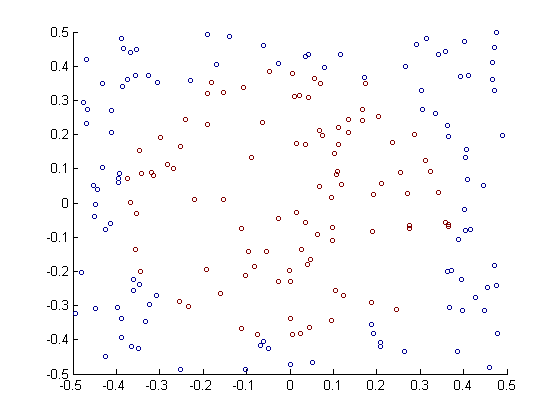
\includegraphics[scale=0.75]{perzeptron5.png}
	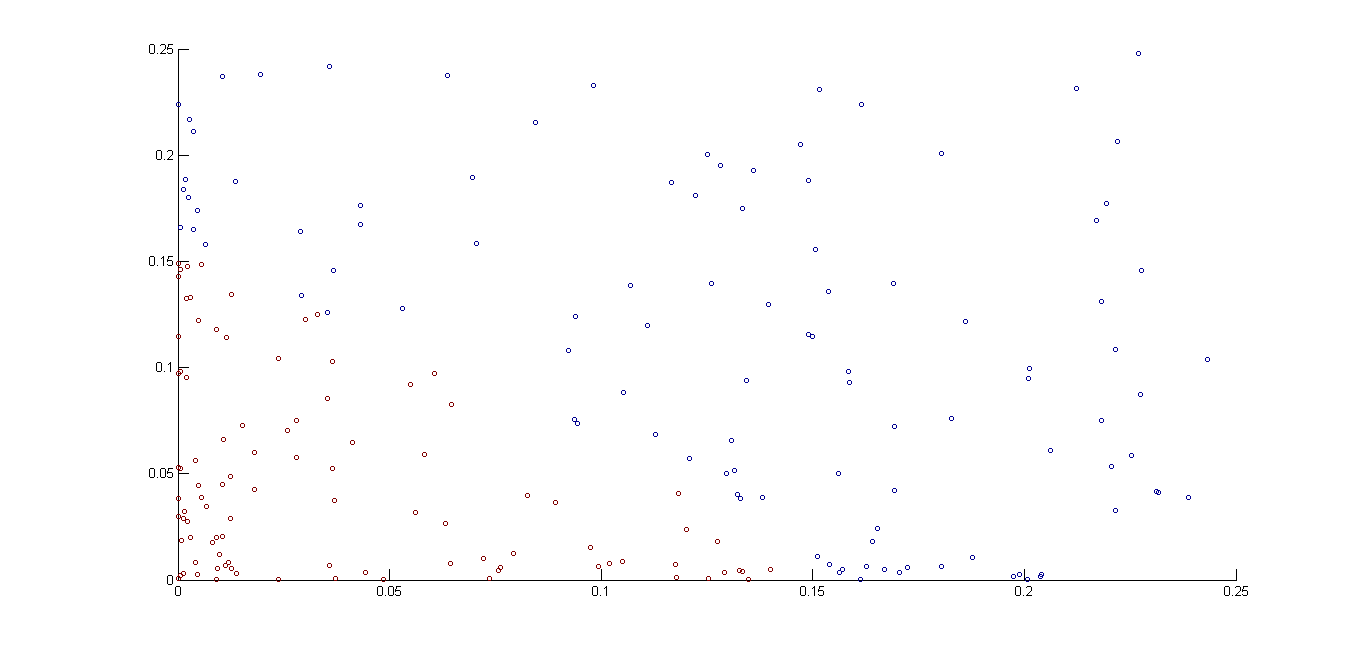
\includegraphics[scale=0.35]{perzsurprise.png}
\end{minipage}
\newline

\subsection*{Perzeptrontraining}

Die Lernrate hat keinen Einfluss für $w_0=0$, da dann $w_i=\gamma * \sum_j{v_j}=0$ mit Vektoren $v_j=x_j * t_j$. Aufgrund der Normierung von $w$ ist die Lernrate irrelevant.


\end{document}          
